% !TEX root = ../notes_template.tex
\chapter{Vectors}\label{chp:vectors}

% \minitoc

\section{$n$-Vectors}
A collection of an ordered list of $n$ numbers is called an $n$-vector. We will use bold lower case alphabets to represent such vectors, and we will represent these as a column of numbers, which is referred to as a \textit{column vector}. We will look at \textit{row vectors} at a later stage. Consider the following example:
\[ \mf{x} = \bmxc x_1 \\ x_2 \\ \vdots \\x_n \emx \]

The elements of the $n$-vector $x_1, x_2, \ldots, x_n$ are called the \textit{components} of the vector $\mf{x}$; $x_i$ is the $i^{th}$ component of the vector $\mf{x}$. If these components are all real numbers, the set of all such $n$-vectors is the set $\mb{R}^n$.

\noindent \textbf{Where do we come across such $n$-vectors?} In many places, such as in physics, engineering, economics, medicine, etc. Any application where we deal with multiple pieces of information that can be represented as a list of numbers can be represented as an $n$-vector. When we deal with systems with multiple inputs, multiple output, or multiple states, we can represent these as $n$-vectors. We talk about the state of a system in a later chapter.

\section{Visualizing $n$-vectors}
The $n$-vectors can be visualized as points in $n$-dimensional space. For example, A 1-vector or just single real number or a \textit{scalar} can be thought of as a point on the real line. The 1-vector $x = 2.45$ is shown in Figure~\ref{fig:1-vector} is the red point. But we will find it useful to visualize a 1-vector as an arrow starting at the origin and ending at the point on the real line. The arrow is shown in blue in Figure~\ref{fig:1-vector}. 

\begin{figure}[b]
    \centering
    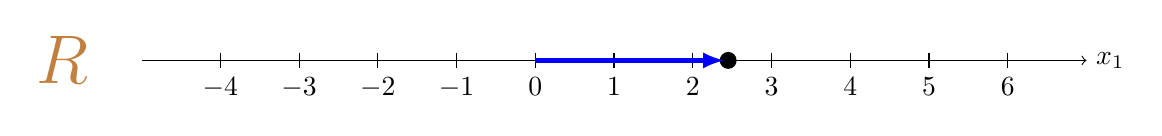
\begin{tikzpicture}
        \draw[->] (-5,0) -- (7,0) node[right] {$x_1$};
        \foreach \x in {,-4,-3,-2,0,-1,1,2,3,4,5,6}
            \draw (\x,0.1) -- (\x,-0.1) node[below] {$\x$};
        % Plot an example point and its corresponding arrow
        \draw[fill=black] (2.45,0) circle (0.1); % Smaller marker size
        \draw[-latex, ultra thick, blue] (0,0) -- (2.4,0); % Thicker arrow
        % Huge font for the label with brown color
        \node[font=\Huge, text=brown] at (-6, 0) {$\mathbb{R}$};
    \end{tikzpicture}
    \caption{The real line $\mb{R}$ contains the $1$-vectors.}
    \label{fig:1-vector}
\end{figure}

The elements of $\mb{R}^2$ are points on the plane, and we can visualize them as points in the plane. The 2-vectors $\mf{x} = \bmxc 2 \\ 3 \emx$ and $\mf{x} = \bmxc -3 \\ 1 \emx$ are shown in Figure~\ref{fig:2-vector}. A similar visualization is shown for $\mb{R}^3$ (Figure~\ref{fig:3-vector}), and for $\mb{R}^4$ and beyond you simply pretend that you can visualize things in your head like your instructor does.

\begin{figure}[t]
    \centering
    \begin{subfigure}[b]{0.45\textwidth}
        \centering
        \begin{tikzpicture}[scale=0.6]
            \draw[->, gray] (-5,0) -- (5,0) node[right] {$x_1$};
            \draw[->, gray] (0,-5) -- (0,5) node[above] {$x_2$};
            \foreach \x in {-4,-2,-1,2,4}
            \draw (\x,0.1) -- (\x,-0.1) node[below, gray] {$\x$};
            \foreach \y in {-4,-2,-1,2,4}
            \draw (0.1,\y) -- (-0.1,\y) node[left, gray] {$\y$};
            % Plot an example point and its corresponding arrow
            \draw[fill=black] (2,3) circle (0.1); % Marker for the point (2,3)
            \draw[-latex, ultra thick, blue] (0,0) --  (2,3) node[right, black] {$\mathbf{x} = \begin{bmatrix} 2 \\ 3 \end{bmatrix}$}; % Arrow with label
            
            \draw[fill=black] (-3,1) circle (0.1); % Marker for the point (-2,1)
            \draw[-latex, ultra thick, red] (0,0) --  (-3,1) node[left, black] {$\mathbf{y} = \begin{bmatrix} -3 \\ 1 \end{bmatrix}$}; % Arrow with label
            
            % Huge font for the label with brown color
            \node[font=\Huge, text=brown] at (-4, 4) {$\mathbb{R}^2$};
        \end{tikzpicture}
        \caption{The $\mathbb{R}^2$ plane contains the $2$-vectors.}
        \label{fig:2-vector}
    \end{subfigure}
    \begin{subfigure}[b]{0.45\textwidth}
        \centering
        \tdplotsetmaincoords{60}{120} % Set the view angle
        \begin{tikzpicture}[scale=0.7,tdplot_main_coords] % Set scale and use the main coordinates
            % Axis lines
            \draw[->, gray] (-5,0,0) -- (5,0,0) node[anchor=north east]{$x_1$};
            \draw[->, gray] (0,-5,0) -- (0,5,0) node[anchor=north west]{$x_2$};
            \draw[->, gray] (0,0,-5) -- (0,0,5) node[anchor=south]{$x_3$};
            \foreach \x in {-4,-2,,2,4}
                \draw (\x,0,0.1) -- (\x,0,-0.1) node[below, gray] {$\x$};
            \foreach \y in {-4,-2,,2,4}
                \draw (0.1,\y,0) -- (-0.1,\y,0) node[above right, gray] {$\y$};
            \foreach \z in {-4,-2,,2,4}
                \draw (0.1,0,\z) -- (-0.1,0,\z) node[above right, gray] {$\z$};
            % Points
            \draw[fill=blue] (1,2,3) circle (0.08);
            \draw[-latex, ultra thick, blue] (0,0,0) --  (1,2,3) node[above, black] {$\mathbf{x} = \bmx 1 \\ 2 \\ 1 \emx$}; 
            % Points
            \draw[fill=red] (2,-1,1) circle (0.08);
            \draw[-latex, ultra thick, red] (0,0,0) --  (2,-1,1) node[below left, black] {$\mathbf{y} = \bmx 2 \\ -1 \\ 1 \emx$}; 
             
            % Huge font for the label with brown color
            \node[font=\Huge, text=brown] at (2,-2,4.5) {$\mathbb{R}^3$};
        \end{tikzpicture}
        \caption{$\mb{R}^3$ contains the 3-vectors.}
        \label{fig:3-vector}
    \end{subfigure}
    \caption{The $\mb{R}^2$ and $\mb{R}^3$ sets.}
    \label{fig:combined}
\end{figure}

\section{Some Commonly Used $n$-vectors}
We will now define a some commonly used $n$-vectors that we will use in the course. 
\begin{itemize}
    \item \textbf{Zero vector:} The $n$-vector whose components are all zeros is called the \textit{zero vector}. $\mf{0} = \bmxc 0 \\ 0 \\ \vdots \\ 0\emx$
    \item \textbf{One vector:} The $n$-vector whose components are all ones is called the \textit{one vector}. $\mf{1} = \bmxc 1 \\ 1 \\ \vdots \\ 1\emx$
    \item \textbf{Unit vectors:} The $n$-vectors whose components are all zeros except for one component which is 1. These are called the \textit{standard basis vectors} and are denoted by $\mf{e}_1, \mf{e}_2, \ldots, \mf{e}_n$. The $n$-vector $\mf{e}_i$ has all components as zeros except for the $i^{th}$ component which is 1. For example, the unit vectors in $\mb{R}^2$ are:
    \[ \mf{e}_1 = \bmx 1 \\ 0\emx \quad \mf{e}_2 = \bmx 0 \\ 1 \emx  \]
\end{itemize}

\section{Operations on $n$-vectors}
There are many operations we can perform on $n$-vectors, but we will only focus on two operations for this:
\begin{itemize}
    \item \textbf{Scalar multiplication:} Given a scalar $c \in \mb{R}$ and an $n$-vector $\mf{x}$. The scalar multiplication operation produces another $n$-vector $c\mf{x}$ whose components are $cx_1, cx_2, \ldots, cx_n$. 
    \[ \mf{x} = \bmx 1 \\ 2\emx \longrightarrow 2 \mf{x} = \bmx  2\ct{1} \\ 2\ct{2} \emx = \bmx  2 \\ 8.2 \emx \]

    The geometric interpretation scalar multiplication is shown in Figure~\ref{fig:scalar-mult}. Scalar multiplication stretches or shrinks the vector without rotating it. When the scalar is positive the direction of the scaled vector is the same as the original vector, and when the scalar is negative the direction is opposite. When the scalar is zero, the scaled vector is the zero vector $\mf{0}$. 
    \begin{figure}[h!]
        \centering
        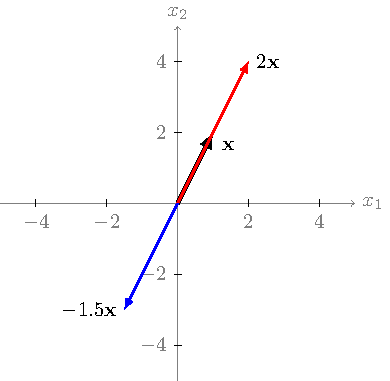
\includegraphics{figure/chapter01/vec-scale.pdf}
        \caption{Scalar multiplication of a vector.}
        \label{fig:scalar-mult}
    \end{figure}
    
    \item \textbf{Vector Addition:} Given two $n$-vectors $\mf{x}$ and $\mf{y}$, the vector addition operation, represented by $\mf{x} + \mf{y}$, producs another $n$-vector whose components are $x_1 + y_1, x_2 + y_2, \ldots, x_n + y_n$.
    \[ \mf{x} = \bmxc 1 \\ 3 \emx, \mf{y} = \bmxc 2 \\ 1 \emx \longrightarrow \mf{x} + \mf{y} = \bmxc 1 + 2 \\ 3 + 1 \emx = \bmxc 3 \\ 4 \emx \]
    
    \begin{figure}[h!]
        \centering
        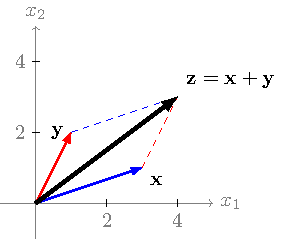
\includegraphics{figure/chapter01/vec-add-fig.pdf}
        \caption{Vector addition.}
        \label{fig:vec-add}
    \end{figure}

    The geometric interpretation the vector addition operation is shown in Figure~\ref{fig:vec-add}. Geometrically, the vector addition operation follows the parallelogram law of addition, where the resulting vector $\mf{x} + \mf{y}$ is a diagonal of the parallelogram formed by the two vectors $\mf{x}$ and $\mf{y}$. Another way to think about this, is that you first move along $\mf{x}$ to its end point, and starting from there then move along $\mf{y}$ to its end point or vice versa.

    You can add more than two vectors to obtain a new vector, like below:
    \[ \mf{w} = \mf{x} + \mf{y} + \mf{z} \]
    Geometrically, we can first apply the parallelogram law to $\mf{x}$ and $\mf{y}$, and then apply the parallelogram law to $\mf{x} + \mf{y}$ and $\mf{z}$ to get $\mf{w}$.
\end{itemize}


\section{Vector spaces}
Vector spaces are \textit{sets} with some special properites. More specifically, a vector space is a set $V$ of elements called \textit{vectors} that are closed under two operations called \textit{addition} and \textit{scalar multiplication}. This simply means that if you perfom these operations using elements from the set $V$, the result is also an element of the set $V$. A vector space must satisfy the following properties:
\begin{itemize}
    \item \textbf{Closure under addition:} For any two vectors $\mf{x}, \mf{y} \in V$, the sum $\mf{x} + \mf{y} \in V$.
    \item \textbf{Closure under scalar multiplication:} For any scalar $c \in \mb{R}$ and any vector $\mf{x} \in V$, the product $c\mf{x} \in V$.
    \item \textbf{Additive identity:} There exists a vector $\mf{0} \in V$ such that for any vector $\mf{x} \in V$, $\mf{x} + \mf{0} = \mf{x}$.
    \item \textbf{Additive inverse:} For any vector $\mf{x} \in V$, there exists a vector $-\mf{x} \in V$ such that $\mf{x} + (-\mf{x}) = \mf{0}$.
    \item \textbf{Commutativity of addition:} For any two vectors $\mf{x}, \mf{y} \in V$, $\mf{x} + \mf{y} = \mf{y} + \mf{x}$.
    \item \textbf{Associativity of addition:} For any three vectors $\mf{x}, \mf{y}, \mf{z} \in V$, $(\mf{x} + \mf{y}) + \mf{z} = \mf{x} + (\mf{y} + \mf{z})$.
    \item \textbf{Distributive property:} For any scalar $c \in \mb{R}$ and any two vectors $\mf{x}, \mf{y} \in V$, $c(\mf{x} + \mf{y}) = c\mf{x} + c\mf{y}$.
    \item \textbf{Distributive property:} For any two scalars $c, d \in \mb{R}$ and any vector $\mf{x} \in V$, $(c + d)\mf{x} = c\mf{x} + d\mf{x}$.
    \item \textbf{Associativity of scalar multiplication:} For any two scalars $c, d \in \mb{R}$ and any vector $\mf{x} \in V$, $(cd)\mf{x} = c(d\mf{x})$.
    \item \textbf{Multiplicative identity:} For any vector $\mf{x} \in V$, $1\mf{x} = \mf{x}$.
\end{itemize}
These properties are satisfied by the set $\mb{R}^n$ of $n$-vectors, and hence $\mb{R}^n$ is a vector space. Geometrically, the concept of a vector space corresponds to flat spaces that contain the origin. This will become more clear when we talk about subspaces. Notice that definition of the vector space given above does not make any specific mention of $n$-vectors. The definition is general and can be applied to any set of elements that satisfy the properties listed above. The following are some examples of vector spaces with the addition and scalar multiplication operations defined on them.

\begin{example}
    \textbf{Set of $m \times n$ matrices.} The set $M$ of all $m \times n$ matrices of real numbers is a vector space.
    \[ \mf{A} = \bmxc
        a_{11} & a_{12} & \cdots & a_{1n} \\
        a_{11} & a_{12} & \cdots & a_{1n} \\
        \vdots & \vdots & \ddots & \vdots \\
        a_{11} & a_{12} & \cdots & a_{1n}
    \emx, \,\, a_{ij} \in \mb{R} \]

    We define scalar multiplication and addition of matrices as follows:
    \[ c\mf{A} = \bmxc
        ca_{11} & ca_{12} & \cdots & ca_{1n} \\
        ca_{11} & ca_{12} & \cdots & ca_{1n} \\
        \vdots & \vdots & \ddots & \vdots \\
        ca_{11} & ca_{12} & \cdots & ca_{1n}
    \emx, \,\, c \in \mb{R} \]
    \[ \mf{A} + \mf{B} = \bmxc
        a_{11} + b_{11} & a_{12} + b_{12} & \cdots & a_{1n} + b_{1n} \\
        a_{11} + b_{11} & a_{12} + b_{12} & \cdots & a_{1n} + b_{1n} \\
        \vdots & \vdots & \ddots & \vdots \\
        a_{11} + b_{11} & a_{12} + b_{12} & \cdots & a_{1n} + b_{1n}
    \emx, \,\, \mf{A}, \mf{B} \in M
    \]
    Since each element of $c\mf{A}$ and $\mf{A} + \mf{B}$ is a real number, $M$ is a vector space.
\end{example}

\begin{example}
    \textbf{Set of polynomials of order $\leq n$.} Now we look at strange example of a vector space. The set $P_n$ of all polynomials of degree at most $n$ with real coefficients, defined over an interval $[a, b]$.
    \[ p\lp x \rp = \sum_{k=0}^{n-1} a_k x^k, \,\, x \in [a, b], \, a_k \in \mb{R} \]
    The set $P_n$ contains all polynomials of the form shown above. We define scalar multiplication and addition of polynomials as follows:
    \[ c p\lp x \rp = c \sum_{k=0}^{n-1} a_k x^k = \sum_{k=0}^{n-1} ca_k x^k, \,\, p\lp x\rp \in P \]
    \[ p\lp x \rp + q\lp x \rp = \sum_{k=0}^{n-1} a_k x^k + \sum_{k=0}^{n-1} b_k x^k = \sum_{k=0}^{n-1} \lp a_k + b_k \rp x^k, \,\, p\lp x \rp, q\lp x \rp \in P_n \]
    The set $P_n$ is a vector space because the sum and product of any two polynomials from $P_n$ is also a polynomial of degree at most $n$ with real coefficients.
\end{example}

\begin{example}
    \textbf{Set of continuous functions.} The set $C\left[0, 1\right]$ of all continuous functions $f\lp x\rp$ over the time interval $x \in \left[ 0, 1\right]$ is a vector space. We define scalar multiplication and addition of functions as follows:
    \[ c f\lp x \rp = c f\lp x \rp, \,\, f\lp x \rp \in C\lp 0, 1 \rp \]
    \[ f\lp x \rp + g\lp x \rp = f\lp x \rp + g\lp x \rp, \,\, f\lp x \rp, g\lp x \rp \in C\lp 0, 1 \rp \]
    The set $C\lp 0, 1 \rp$ is a vector space because the sum and product of any two continuous functions from $C\lp 0, 1 \rp$ is also a continuous function.
\end{example}

\section{Subspaces -- ``Little'' Vector Spaces}
These are little subspaces in the sense that they are subsets of a larger vector space that are themselves vector spaces. More formally, a subspace $U$ of a vector space $V$ is a subset of $V$ that is itself a vector space. The subspace $U$ of the vector space $V$ must satisfy the following properties:
\begin{itemize}
    \item \textbf{Closure under addition:} For any two vectors $\mf{x}, \mf{y} \in U$, the sum $\mf{x} + \mf{y} \in U$.
    \item \textbf{Closure under scalar multiplication:} For any scalar $c \in \mb{R}$ and any vector $\mf{x} \in U$, the product $c\mf{x} \in U$.
\end{itemize}
One immediate consequence of the above definition is that hte zero element of the vector space $V$ must be present in every subspace of $V$. If the zero element is not in a subset, then it cannot be a subspace. Geometrically subspace capture the idea of flat spaces that contain the origin, and extend infinitely. Let's look at some examples of subspaces of $\mb{R}^2$ and $\mb{R}^3$, which are easier to visualize.

\begin{example}
    \textbf{A straight line through the origin.} We know that $\mb{R}^2$ is a vector space. Now consider the set of all points in $\mb{R}^2$ that lie on a straight line passing through the origin, defined as follows:
    \[ S = \lc \mf{x} \, : \, x = \bmx x_1 \\ x_2 \emx \in \mb{R}^2, \, x_1 = m \cdot x_2, \, m \in \mb{R} \rc \]
    How do we verfiy this is a subspace of $\mb{R}^2$? The definition above shows that any $x$ in $S$ comes from $\mb{R}^2$, which means its a subset of $\mb{R}^2$. Figure~\ref{fig:subspace1} shows the set $S$ for $m = 2$.
    \begin{figure}[h]
    \centering
    \begin{subfigure}[b]{0.32\textwidth}
        \begin{tikzpicture}[scale=0.32]
            \draw[->, gray] (-5,0) -- (5,0) node[right] {$x_1$};
            \draw[->, gray] (0,-5) -- (0,5) node[above] {$x_2$};
            \foreach \x in {-4,-2,2,4}
            \draw (\x,0.1) -- (\x,-0.1) node[below, gray] {$\x$};
            \foreach \y in {-4,-2,2,4}
            \draw (0.1,\y) -- (-0.1,\y) node[left, gray] {$\y$};
            % Plot an example point and its corresponding arrow
            \draw[thick, blue] (-2.5,-5) --  (2.5,5);
            \node[right, black] at (1.4, 3) {$S = \left\{ \begin{bmatrix} x \\ 2x \end{bmatrix}\right\}$};
    
            % Huge font for the label with brown color
            \node[font=\Large, text=brown] at (-4, 4) {$\mathbb{R}^2$};
        \end{tikzpicture}
        \caption{A subspace of $\mb{R}^2$.}
        \label{fig:subspace1}
    \end{subfigure}
    \begin{subfigure}[b]{0.32\textwidth}
        \centering
        \begin{tikzpicture}[scale=0.35]
            \draw[->, gray] (-5,0) -- (5,0) node[right] {$x_1$};
            \draw[->, gray] (0,-5) -- (0,5) node[above] {$x_2$};
            \foreach \x in {-4,-2,2,4}
            \draw (\x,0.1) -- (\x,-0.1);
            \foreach \y in {-4,-2,2,4}
            \draw (0.1,\y) -- (-0.1,\y);
            % Plot an example point and its corresponding arrow
            \draw[thick, blue] (-2.5,-5) --  (2.5,5);
            
            \draw[-latex, ultra thick, black!40!green] (0,0) --  (2,4) node[font=\small, right, yshift=-0.0cm, black!40!green] {$2\mathbf{x} = \begin{bmatrix} 2 \\ 4 \end{bmatrix}$}; % Arrow with label
    
            \draw[-latex, ultra thick, red] (0,0) --  (1,2) node[font=\small, right, yshift=-0.25cm, red] {$\mathbf{x} = \begin{bmatrix} 1 \\ 2 \end{bmatrix}$}; % Arrow with label
        \end{tikzpicture}
        \caption{Vector scaling.}
        \label{fig:subspace1-scale}
    \end{subfigure}
    \begin{subfigure}[b]{0.32\textwidth}
        \centering
        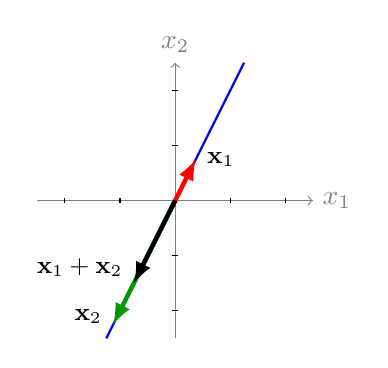
\begin{tikzpicture}[scale=0.35]
            \draw[->, gray] (-5,0) -- (5,0) node[right] {$x_1$};
            \draw[->, gray] (0,-5) -- (0,5) node[above] {$x_2$};
            \foreach \x in {-4,-2,2,4}
            \draw (\x,0.1) -- (\x,-0.1);
            \foreach \y in {-4,-2,2,4}
            \draw (0.1,\y) -- (-0.1,\y);
            % Plot an example point and its corresponding arrow
            \draw[thick, blue] (-2.5,-5) --  (2.5,5);
            
            \draw[-latex, ultra thick, black!40!green] (0,0) --  (-2.25,-4.5) node[font=\small, left, yshift=0.1cm, black] {$\mathbf{x}_2$}; % Arrow with label
            
            \draw[-latex, ultra thick, red] (0,0) --  (0.75,1.5) node[font=\small, right, yshift=0.0cm, black] {$\mathbf{x}_1$}; % Arrow with label
            
            \draw[-latex, ultra thick, black] (0,0) --  (-1.5,-3.0) node[font=\small, left, yshift=0.2cm, black] {$\mathbf{x}_1 + \mathbf{x}_2$}; % Arrow with label
        \end{tikzpicture}
        \caption{Vector addition.}
        \label{fig:subspace1-addition}
    \end{subfigure}
    \caption{Example of a subspace of $\mb{R}$. (a) Shows the set of all points in $\mb{R}^2$ corresponding to the subset $S = \left\{ \bmxc x \\ 2 x\emx\right\} \subset \mb{R}^2$. (b) Shows that the set $S$ is closed under scalar multiplication. Take any vecotr from the line, and scale it and it remains on that blue line. (c) Shows that $S$ is closed under vector addition. If we take any two vectors from the blue line and add them, the resulting vector remains in the blue line.}
    \end{figure}    

    \noindent How do we verify if $S$ is a subspace of $\mb{R}^2$? We need to now verify that $S$ satisfies the properties of a vector space.
    \begin{enumerate}
        \item First, let's check if $S$ contains the zero vector. If it does not contain the zero vector, then it cannot be a subspace. The elements from $S$ are of the form $\bmxc x \\ m x\emx$, thus if we choose $x = 0$, then we get $\bmx 0 \\ 0 \emx \in S$. So, $S$ contains the zero vector. This means that $S$ can be a subspace space of $\mb{R}^2$.
        \item Let's verify vector scaling. Scaling the element $\bmxc x \\ m x \emx \in S$ by a scalar $c$ we get,
        \[ c \bmxc x \\ m x\emx = \bmxc c x \\ c m x \emx = \bmxc c x \\ m \pp{c x} \emx = \bmxc y \\ m y\emx, \quad \text{where} \,\, y = c x \in \mb{R} \]
        This means that $c\bmxc x \\ m x\emx$ belongs to $S$, this the set $S$ is closed under scalar multiplication. This still means that $S$ can be a subspace of $\mb{R}^2$.
        \item Let's verify vector addition. Adding two elements $\bmxc x_1 \\ m x_1\emx, \bmxc x_2 \\ m x_2\emx \in S$ we get,
        \[ \bmxc x_1 \\ m x_1\emx + \bmxc x_2 \\ m x_2\emx = \bmxc x_1 + x_2 \\ m x_1 + m x_2 \emx = \bmxc y_1 \\ m y_1\emx, \quad \text{where} \,\, y_1 = x_1 + x_2 \in \mb{R} \]
        This means that $\bmxc y_1 \\ m y_1\emx$ belongs to $S$, this the set $S$ is closed under vector addition. This means that $S$ is a subspace of $\mb{R}^2$.
    \end{enumerate}
    Since, the subset $S$ is closed under both vector addition and scalar multiplication, it is a subspace of $\mb{R}^2$.
\end{example}

\begin{example}
    \textbf{A straight line not through the origin.} Consider the set of all points in $\mb{R}^2$ of the following form:
    \[ S = \lc \mf{x} \, : \, x = \bmxc x \\ m x + c \emx \in \mb{R}^2, \, m, c \in \mb{R} \rc \]
    This is shown in the Figure~\ref{fig:subspace2}
    How do we verfiy this is a subspace of $\mb{R}^2$? The definition above shows that any $x$ in $S$ comes from $\mb{R}^2$, which means its a subset of $\mb{R}^2$. Figure~\ref{fig:subspace1} shows the set $S$ for $m = 2$.
    \begin{figure}[h!]
    \centering
    \begin{tikzpicture}[scale=0.4]
        \draw[->, gray] (-5,0) -- (5,0) node[right] {$x_1$};
        \draw[->, gray] (0,-5) -- (0,5) node[above] {$x_2$};
        \foreach \x in {-4,-2,2,4}
        \draw (\x,0.1) -- (\x,-0.1) node[below, gray] {$\x$};
        \foreach \y in {-4,-2,2,4}
        \draw (0.1,\y) -- (-0.1,\y) node[left, gray] {$\y$};
        % Plot an example point and its corresponding arrow
        \draw[thick, blue] (-5,3) --  (5,-2.0);
        \node[right, black] at (2.25, 4) {$S = \left\{ \begin{bmatrix} x \\ -2x + \frac{1}{2} \end{bmatrix} \,\, : \,\, x \in \mb{R} \right\}$};
        % Huge font for the label with brown color
        \node[font=\Large, text=brown] at (-4, 4) {$\mathbb{R}^2$};
    \end{tikzpicture}
    \caption{Not a subspace of $\mb{R}^2$.}
    \label{fig:subspace2}
    \end{figure}
    \noindent How do we verify if $S$ is a subspace of $\mb{R}^2$? We need to now verify that $S$ satisfies the properties of a vector space.
    \begin{enumerate}
        \item First, let's check if $S$ contains the zero vector. If it does not contain the zero vector, then it cannot be a subspace. The elements from $S$ are of the form $\bmxc x \\ m x\emx$, thus if we choose $x = 0$, then we get $\bmx 0 \\ 0 \emx \in S$. So, $S$ contains the zero vector. This means that $S$ can be a subspace space of $\mb{R}^2$.
        \item Let's verify vector scaling. Scaling the element $\bmxc x \\ m x \emx \in S$ by a scalar $c$ we get,
        \[ c \bmxc x \\ m x\emx = \bmxc c x \\ c m x \emx = \bmxc c x \\ m \pp{c x} \emx = \bmxc y \\ m y\emx, \quad \text{where} \,\, y = c x \in \mb{R} \]
        This means that $c\bmxc x \\ m x\emx$ belongs to $S$, this the set $S$ is closed under scalar multiplication. This still means that $S$ can be a subspace of $\mb{R}^2$.
        \item Let's verify vector addition. Adding two elements $\bmxc x_1 \\ m x_1\emx, \bmxc x_2 \\ m x_2\emx \in S$ we get,
        \[ \bmxc x_1 \\ m x_1\emx + \bmxc x_2 \\ m x_2\emx = \bmxc x_1 + x_2 \\ m x_1 + m x_2 \emx = \bmxc y_1 \\ m y_1\emx, \quad \text{where} \,\, y_1 = x_1 + x_2 \in \mb{R} \]
        This means that $\bmxc y_1 \\ m y_1\emx$ belongs to $S$, this the set $S$ is closed under vector addition. This means that $S$ is a subspace of $\mb{R}^2$.
    \end{enumerate}
    Since, the subset $S$ is closed under both vector addition and scalar multiplication, it is a subspace of $\mb{R}^2$.
\end{example}


% The addition operation takes two vectors and produces another vector in the set, and the scalar multiplication operation takes a scalar and a vector and produces another vector in the set. The set $V$ must satisfy the following properties:

% There are many operations we can perform on $n$-vectors, but we will only focus on two operations for this:
% \begin{itemize}
%     \item \textbf{Scalar multiplication:} Given a scalar $c \in \mb{R}$ and an $n$-vector $\mf{x}$. The scalar multiplication operation produces another $n$-vector $c\mf{x}$ whose components are $cx_1, cx_2, \ldots, cx_n$. 
%     \[ \mf{x} = \bmx 1 \\ 2\emx \longrightarrow 2 \mf{x} = \bmx  2\ct{1} \\ 2\ct{2} \emx = \bmx  2 \\ 8.2 \emx \]

%     The geometric interpretation scalar multiplication is shown in Figure~\ref{fig:scalar-mult}. Scalar multiplication stretches or shrinks the vector without rotating it. When the scalar is positive the direction of the scaled vector is the same as the original vector, and when the scalar is negative the direction is opposite. When the scalar is zero, the scaled vector is the zero vector $\mf{0}$. 
%     \begin{figure}[h!]
%         \centering
%         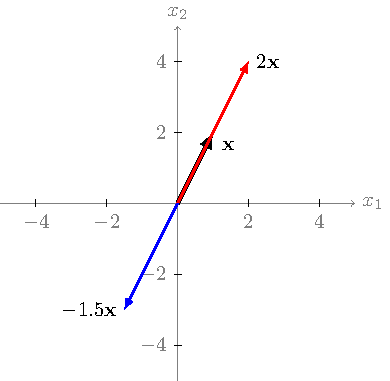
\includegraphics{figure/chapter01/vec-scale.pdf}
%         \caption{Scalar multiplication of a vector.}
%         \label{fig:scalar-mult}
%     \end{figure}
    
%     \item \textbf{Vector Addition:} Given two $n$-vectors $\mf{x}$ and $\mf{y}$, the vector addition operation, represented by $\mf{x} + \mf{y}$, producs another $n$-vector whose components are $x_1 + y_1, x_2 + y_2, \ldots, x_n + y_n$.
%     \[ \mf{x} = \bmxc 1 \\ 3 \emx, \mf{y} = \bmxc 2 \\ 1 \emx \longrightarrow \mf{x} + \mf{y} = \bmxc 1 + 2 \\ 3 + 1 \emx = \bmxc 3 \\ 4 \emx \]
    
%     \begin{figure}[h!]
%         \centering
%         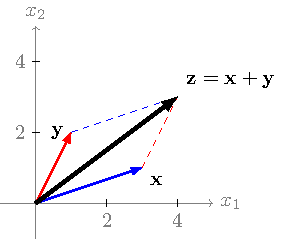
\includegraphics{figure/chapter01/vec-add-fig.pdf}
%         \caption{Vector addition.}
%         \label{fig:vec-add}
%     \end{figure}

%     The geometric interpretation the vector addition operation is shown in Figure~\ref{fig:vec-add}. Geometrically, the vector addition operation follows the parallelogram law of addition, where the resulting vector $\mf{x} + \mf{y}$ is a diagonal of the parallelogram formed by the two vectors $\mf{x}$ and $\mf{y}$. Another way to think about this, is that you first move along $\mf{x}$ to its end point, and starting from there then move along $\mf{y}$ to its end point or vice versa.

%     You can add more than two vectors to obtain a new vector, like below:
%     \[ \mf{w} = \mf{x} + \mf{y} + \mf{z} \]
%     Geometrically, we can first apply the parallelogram law to $\mf{x}$ and $\mf{y}$, and then apply the parallelogram law to $\mf{x} + \mf{y}$ and $\mf{z}$ to get $\mf{w}$.
% \end{itemize}



% gls example
% \begin{itemize}
% 	% \item \glsxtrshort{gcd};
% 	\item \Gls{gcd}; \acrlong{gcd}; \acrshort{gcd}; \acrfull{gcd}
% \end{itemize}

% \section{Proof}
% \begin{lemma}
% \end{lemma}
% \begin{claim}
% \end{claim}
% \begin{theorem}
% \end{theorem}
% \begin{example}
% \end{example}
% \begin{fact}
% \end{fact}
% \begin{remark}
% \end{remark}
% \begin{exercise}
% 	Prove A \iff B
% \end{exercise}
% \begin{solution}
% By induction:
% \end{solution}

% \lipsum % dummy text - remove from real document

% \section{Quantifier}
% \lipsum % dummy text - remove from real document

% \section{Graph}
% \citetitle{babaiGraphIsomorphismQuasipolynomial2016}
% \cite{babaiGraphIsomorphismQuasipolynomial2016}

\section{Number theory}
Figure example
\begin{figure}[!ht]
    \centering
    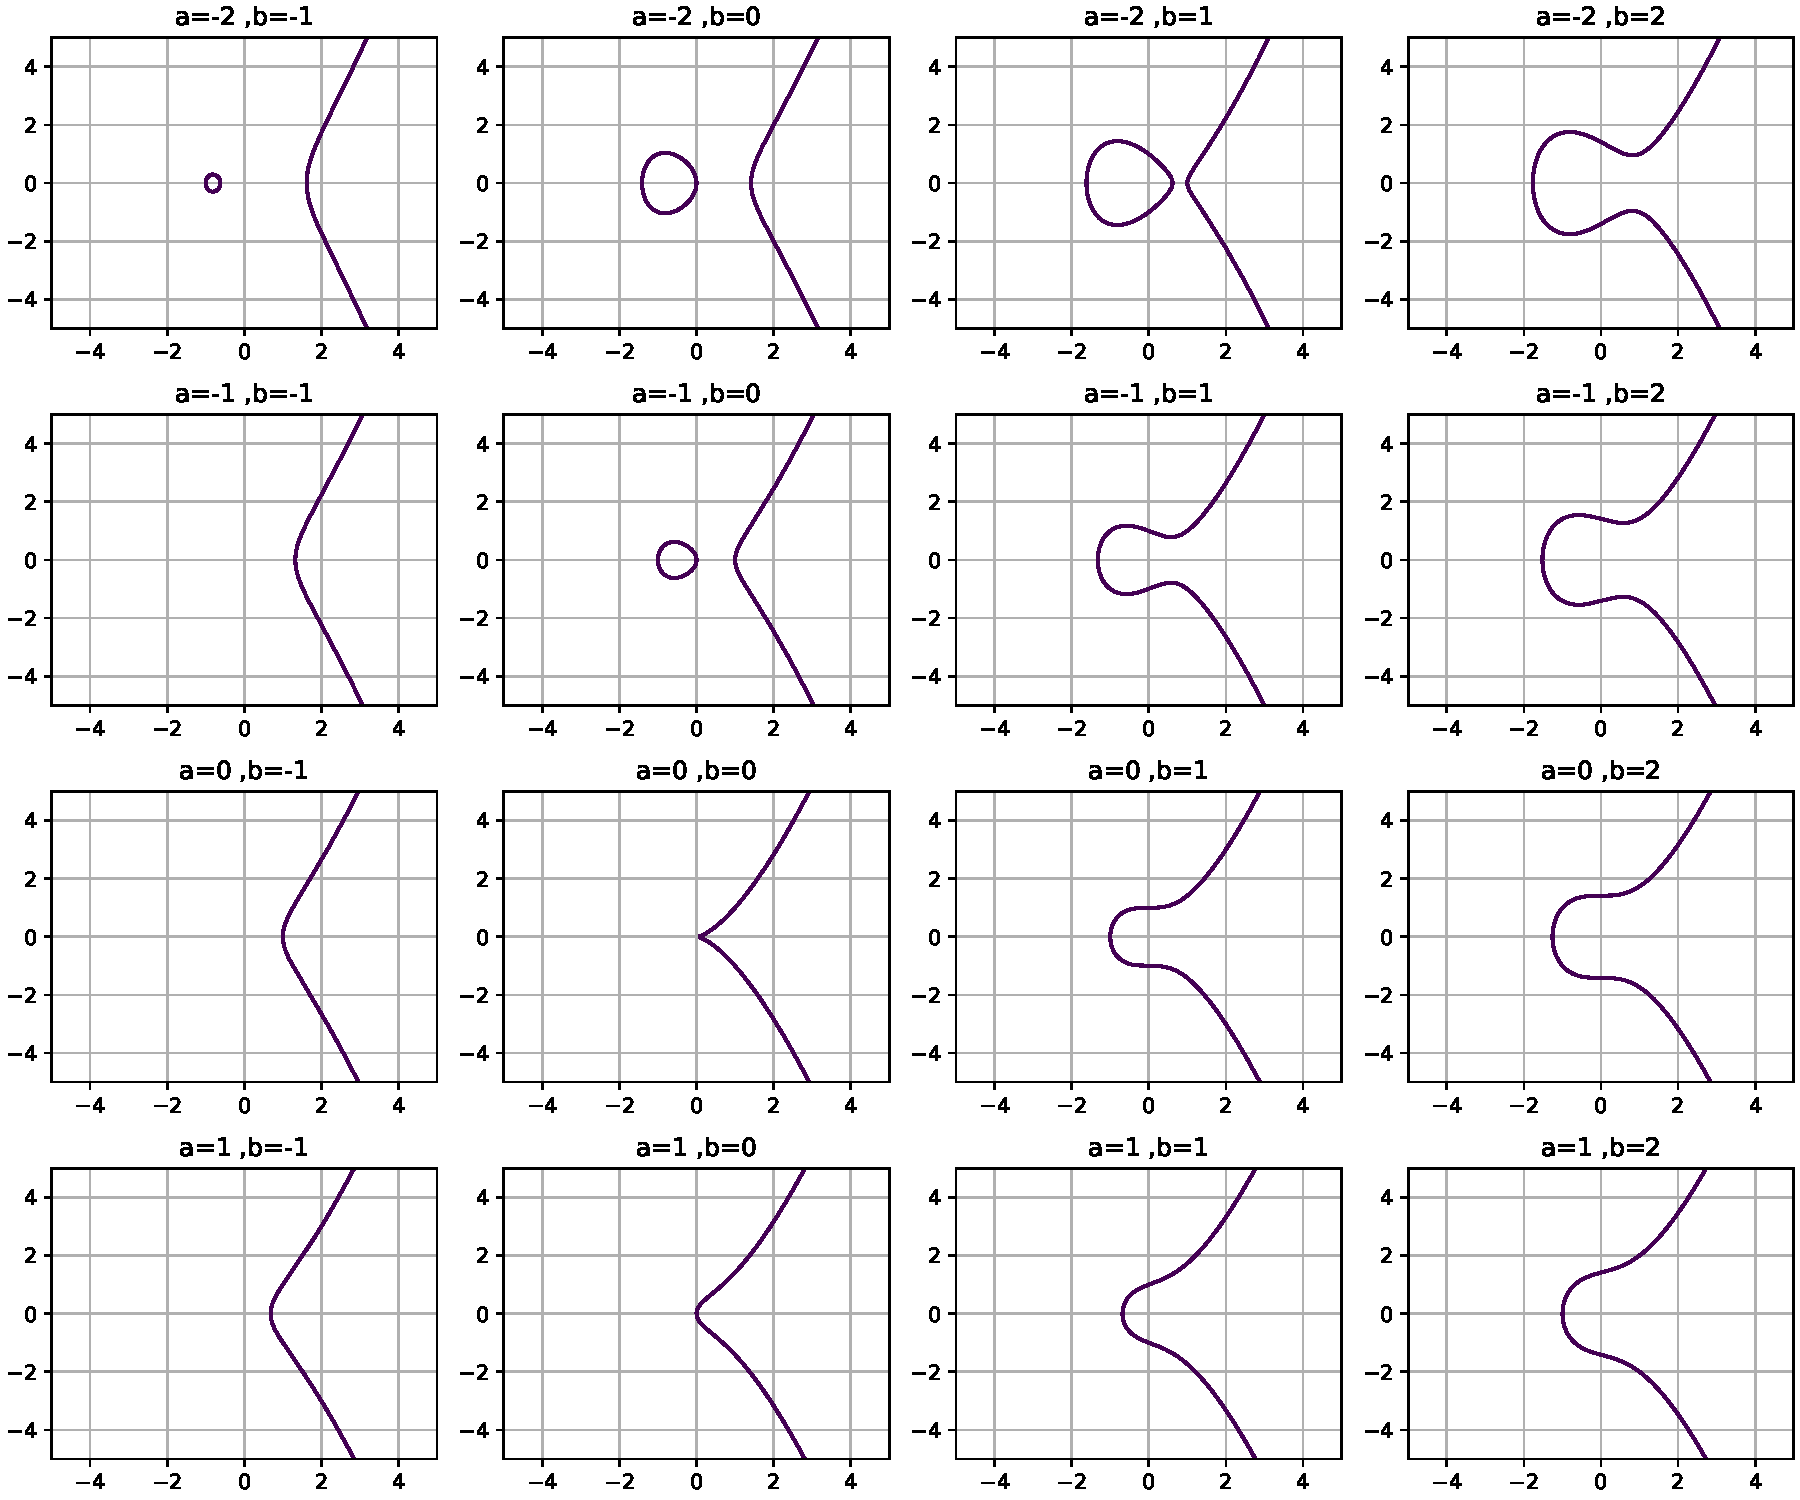
\includegraphics[width=1\linewidth]{./figure/elliptic_curves.pdf}
    \caption{Elliptic curves \cite{childsUniversalComputationQuantum2009} }
\end{figure}


\section{Algorithm}
% \begin{center}
% \begin{minipage}{.9\linewidth}
% algorithm2e
% https://www.overleaf.com/learn/latex/Algorithms#The_algorithm2e_package
\begin{algorithm}[H]
    \SetKwInOut{Input}{input}
    \SetKwInOut{Output}{output}
    \Input{Integer $N$ and parameter $1^t$}
    \Output{A decision as to whether $N$ is prime or composite}
    \BlankLine
    \For{ $i = 1,2, \ldots, t$} {
        $a\leftarrow \qty{1,\dots,N_1}$\;
        \If{$a^{N-1} \neq 1 \mod{N}$}
    {\Return "composite"}
    }
    \Return "prime"
    \caption{Primality testing - first attempt}
    \label{alg:miller_rabin}
\end{algorithm}
% \end{minipage}
% \end{center}